\section{Architektur}

\begin{figure}[ht]
		\centering
		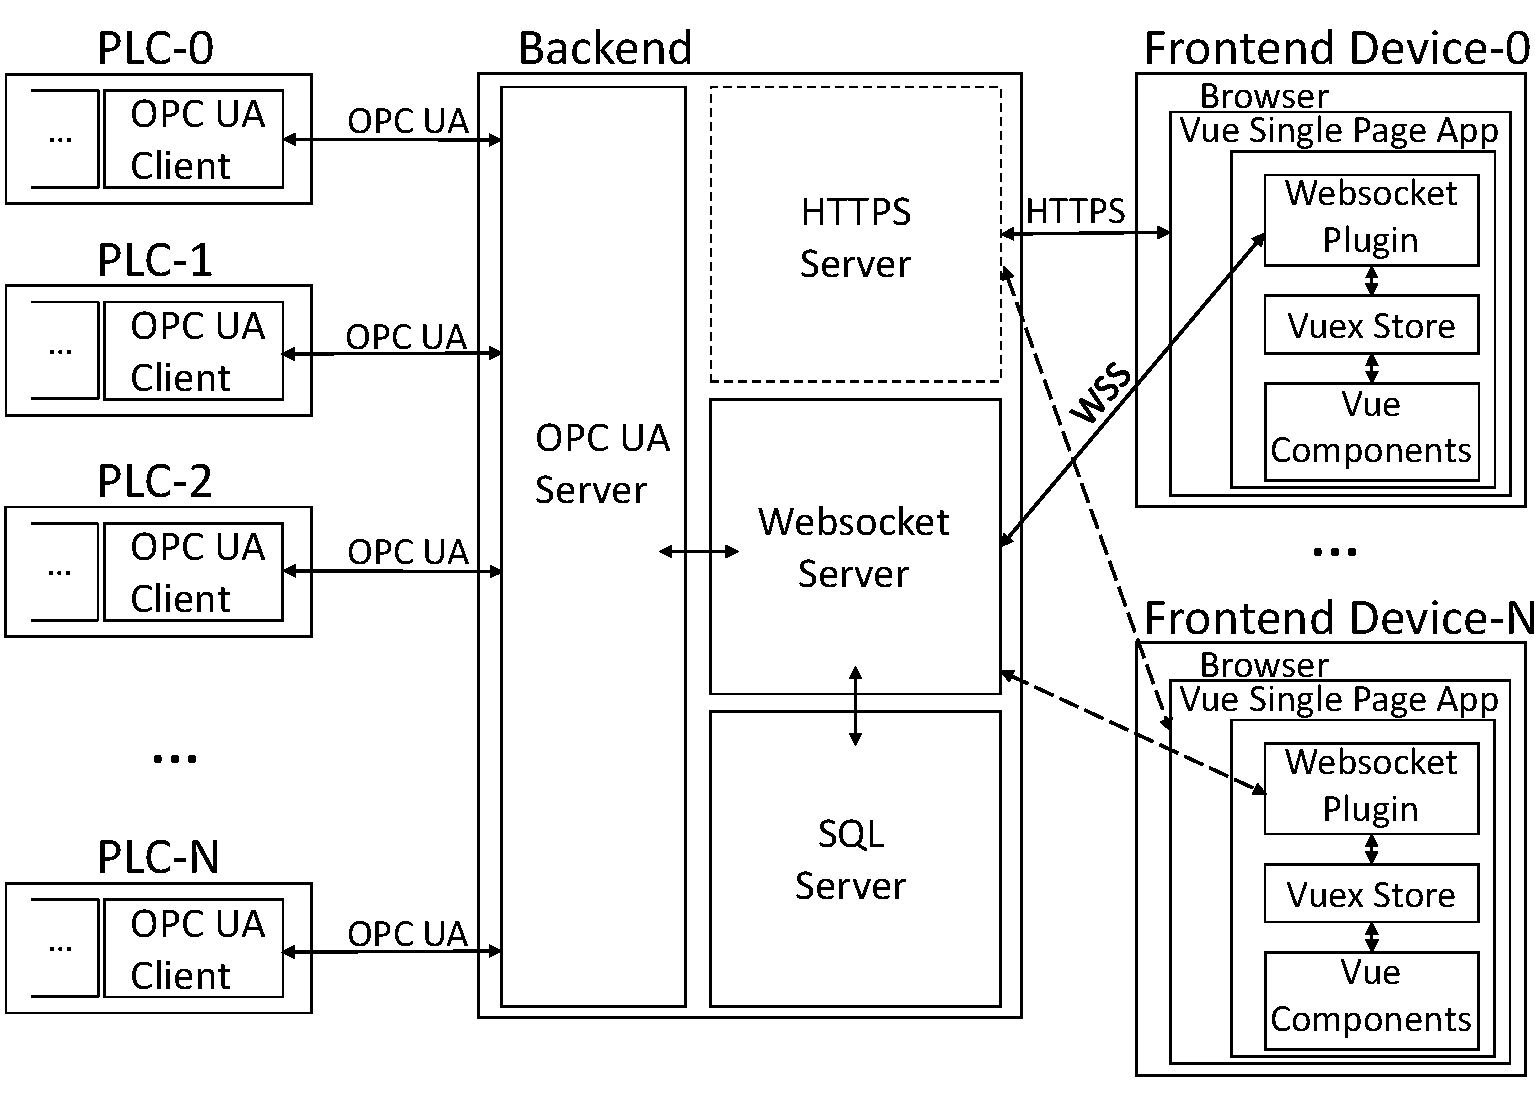
\includegraphics[width=\textwidth]{content/hauptteil/systemEntwurf/res/comMod.pdf}
    \caption[Kommunikationsmodell des \acs{scada} Systems]{Kommunikationsmodell des \acs{scada} Systems.\\
      Die CPUs sind per \acs{opcua} an das Scada System angebunden und haben die Rolle eines \acs{opcua} Clients.
      Die Webapplikation im Browser kommuniziert über \acs{wss} sowie \acs{https} verschlüsselt mit dem Backend.}
		\label{img:comMod}
\end{figure}
Wie in Abbildung \ref{img:comMod} dargestellt, lässt sich die Architektur des \ac{scada} Systems in \acp{plc} Backend und Frontend unterteilen.
Unter Frontend (Abschnitt \ref{subsec:archFrontend})versteht man die (in diesem Fall) grafische Schnittstelle, 
die es dem Nutzer ermöglicht mit dem System zu interagieren.
Das Backend (Abschnitt \ref{subsec:archBackend}) fasst den Rest des Systems zusammen.
\subsection{Backend}\label{subsec:archBackend}
Das Backend besteht aus den folgenden vier Komponenten:
 \begin{itemize}
  \item Einem \ac{https} Server
  \item Einem \ac{wss} Server 
  \item Einem \ac{sql} Server
  \item Einem \ac{opcua} Server 
\end{itemize}
Damit ergeben sich, wenn man das Backend von außen betrachtet, als Schnittstellen \ac{opcua}, \ac{wss} und \ac{https}.
Über diese Schnittstellen stellt das Backend den \acp{plc} sowie dem Frontend, Services zur Verfügung.
Eine Sonderolle unter den Komponenten nimmt dabei der \ac{https} Server ein, 
da er als einzigste keine Verbindung mit dem Rest des Backends hat.
Dies ist deshalb möglich, da der \ac{https} Server dazu da ist, die \ac{html}, die \ac{css}, sowie die \ac{js} Dokumente 
einmalig beim Seitenaufruf an das Endgerät (Frontend Host Device) auszuliefern.
Von diesem Zeitpunkt ab findet die Kommunikation zwischen Frontend und Backend ausschließlich über den \ac{wss} Server statt.
Zwischen dem Websocket Server und dem Frontend können von da an Strings ausgetauscht werden.
Der \ac{opcua} Server hält die variablen Daten des Systems und bietet diese den angeschlossenen \acp{plc} an.
Die Parametrierung des Frontends sowie alle anderen Daten die persistiert werden müssen, 
werden in einem \ac{sql} Server in Form einer relationalen Datenbank gespeichert.
\subsection{Frontend}\label{subsec:archFrontend}
Das Frontend ist eine \ac{html} Webapplikation,
\dots
\section{Datenstruktur}
\begin{figure}[ht]
  \centering
  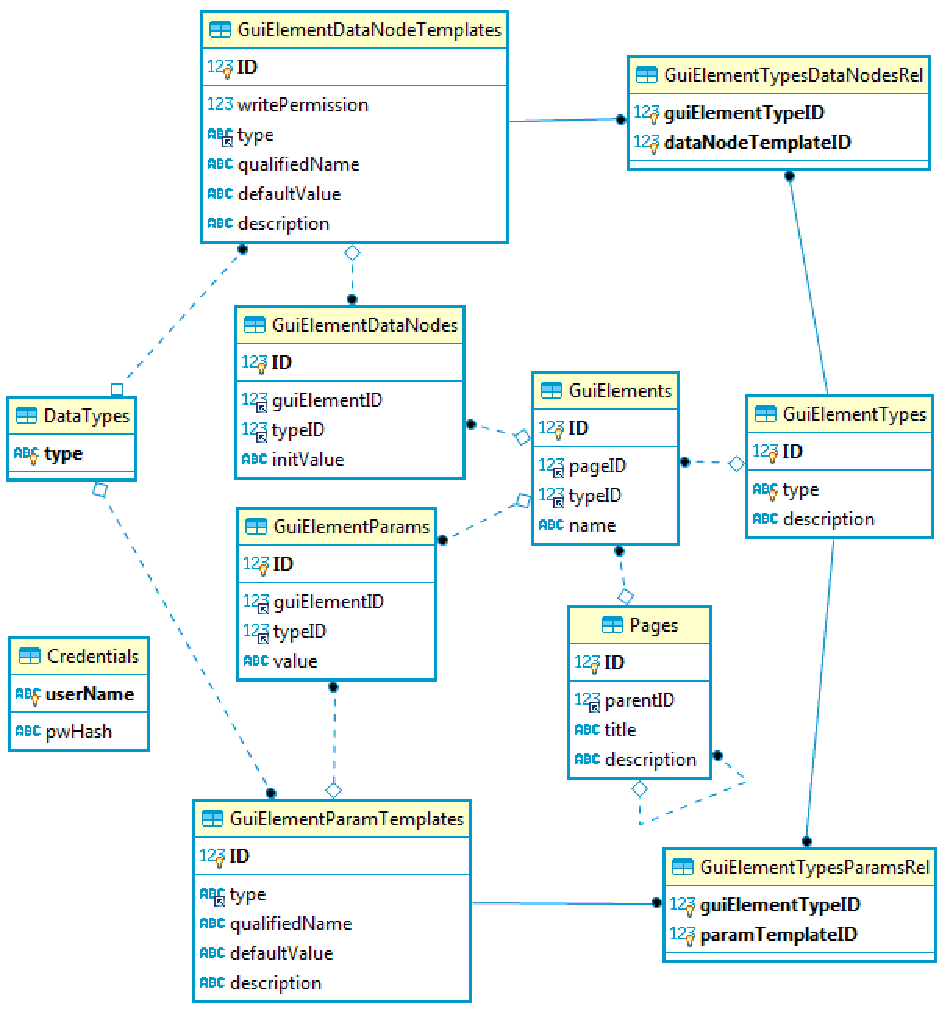
\includegraphics[width=\textwidth]{content/hauptteil/systemEntwurf/res/erd.pdf}
  \caption[\acs{erd} des \acs{scada} Systems]{\acs{erd} des \ac{scada} Systems.\\
    Darstellung zeigt die einzelnen Tabellen der Datenbank auf dem \ac{sql} Server und deren Beziehungen zueinander.}
  \label{img:erd}
\end{figure}
Das abgebildete \ac{erd} in Abbildung \ref{img:erd}, stellt die globale Datenstruktur der Datenbank auf dem \ac{sql} Server dar.
Sie besteht aus einzelnen Tabellen deren Primärschlüssel ausgenommen einzelner Hilfstabellen immer eine ID ist.
Zentrales Element sind dabei die \ac{gui} Elemente (Tabelle \emph{GuiElements}). Jedes \ac{gui} Element ist einer Page (Tabelle \emph{Pages}) zugeordnet. 
Eine Page kann wiederum einer anderen Page zugeordnet sein. 
Dies wird erreicht indem jeder Page Datensatz eine ParentID enthält, welche als Fremdschlüssel auf die übergeordnete Page zeigt. So entsteht eine Baumstruktur innerhalb der Entitäten.
Ist der Wert dieses Fremdschlüssels \emph{NULL} so hat die jeweilige Page keine übergeordnete Page und liegt damit im Wurzelverzeichnis.\\
Jedes \ac{gui} Element hat n Parameter und m Data Nodes (mit $ n, m \in \N $). 
Diese werden in den Tabellen \emph{GuiElementParams} sowie \emph{GuiElementDataNodes} verwaltet.
Jede DataNode, beziehungsweise jeder Parameter, hat einen Datentyp ein Namen, eine Beschreibung, sowie einen Wert. 
Bei den Parametern entspricht dies dem tatsächlichen aktuellen Wert, 
bei den DataNodes entspricht dies dem initialen Wert beim Starten des Backends.
Die zuvor beschriebenen \ac{gui} Elemente besitzen außerdem einen Typ (verwaltet in der Tabelle \emph{GuiElementTypes}).
Jedem Typ sind nun n DataNodeTemplates (Tabelle \emph{GuiElementDataNodeTemplates}) zugeordnet, 
aus denen die eigentlichen Datanodes beim Instanzieren erstellt werden. Da eine solche Vorlage für DataNodes auch für mehrere \ac{gui} Element Typen verwendet werden kann, ist die Verbindung eine n:m Bindung. 
Dies ist in einer Datenbank nur durch eine Hilfstabelle, 
welche die Primärschlüssel zweier Tabellen miteinander verknüpft, ereichbar. 
Analog zu den DataNodes ist der gleiche Mechanismus für die Parameter vorgesehen.
Um ein sauberes Interface zu schaffen sind zum Instanzieren, 
sowie zum Löschen der \ac{gui} Elemente, Stored Procedures vorgesehen.
Die komplette Datenstruktur des \ac{sql} Servers ist so abgelegt, 
dass er alle relevanten Relationen kennt und entsprechend verwaltet.
So wird beispielsweise beim Löschen eines \ac{gui} Elements alle zugehörigen DataNodes mitgelöscht und 
beim Löschen einer kompletten Page werden alle der Page zugeordneten \ac{gui} Elemente auch gelöscht (\emph{on delete cascade}, Abschnitt \ref{subsec:relDB}).\\ \\

Der \ac{opcua} Server hält alle DataNodes der \ac{gui} Elemente. 
Diese \ac{gui} Elemente werden entsprechen der Pages, denen sie zugeordnet sind, auf dem \ac{opcua} Server abgelegt und 
sind den \acp{plc} dort zugänglich.
Ob eine DataNode von den \acp{plc} nur gelesen oder auch beschrieben werden kann, 
wird durch das Flag \emph{writePermission} auf dem \ac{sql} Server in der DataNodeTemplate Tabelle festgelegt. 
Beim Erstellen der DataNode auf dem \ac{opcua} Server, wird dieses Flag ausgelesen und 
direkt in die Konfiguration des \ac{opcua} Servers übernommen.
Der native Datentyp mit dem die DataNodes auf dem \ac{opcua} Server abgelegt werden, wird den DataNodeTemplates des \ac{sql} Servers entnommen.

Auf dem \ac{sql} Server haben die DataNodes sowie Parameter immer den native \ac{sql} Datentyp \emph{VARCHAR} um ein Speicherfeld zu erhalten, dass alle benutzten \ac{opcua} Datentypen unterstützt.
Beim Lesen beziehungsweise beim Schreiben wird als String gespeicherte wert auf dem \ac{sql} Server, 
entsprechend seines explizit abgespeicherten Typs, konvertiert. 
%hier noch mehr entry: OPCUASERVER::createDataNode(MYSQL_RES) aber: abstract ohne auf impl einzugehn
GuiElements und Pages haben als Datentyp auf dem \ac{opcua} Server den Typ BaseObjectType.
Auf einen Spezialisierung dieser Typdefinition für Pages und \ac{gui} Elements auf dem \ac{opcua} Server wird absichtlich verzichtet, 
da sie nur zur Strukturierung der DataNodes genutzt werden.







\begin{figure}
  \centering
  \begin{subfigure}[b]{0.48\textwidth}
    \centering
    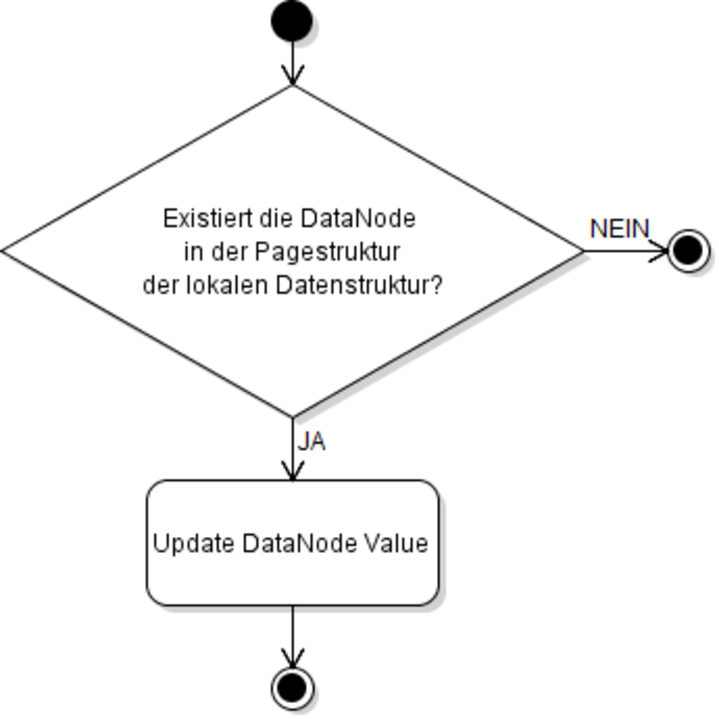
\includegraphics[width=\textwidth]{content/hauptteil/systemEntwurf/res/wsHandler/frontend/wsEvent_dataNodeChange.pdf}
    \caption{WebsocketEvent:\\\emph{DataNodeChange} empfangen}
    \label{fig:aDDF:wsEvent_dataNodeChange}
  \end{subfigure}
  \hfill
  \begin{subfigure}[b]{0.48\textwidth}
      \centering
      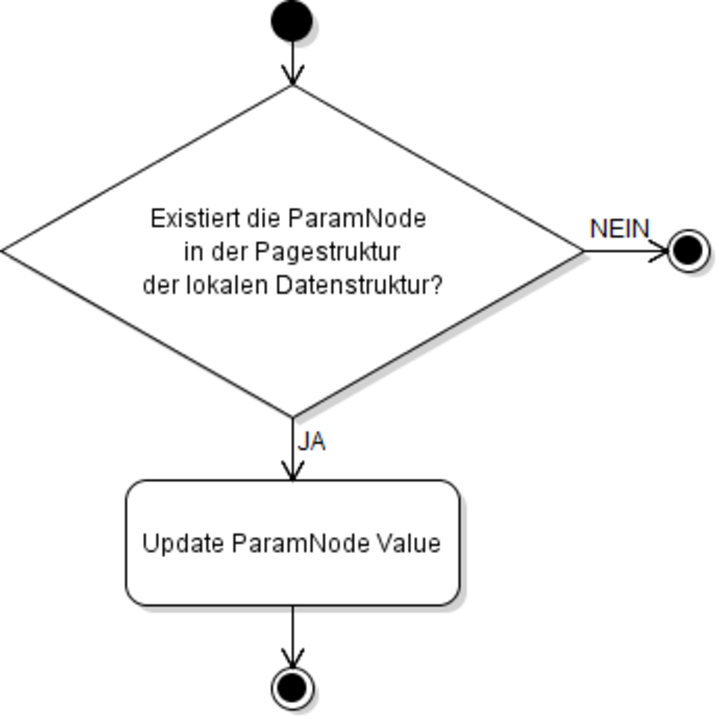
\includegraphics[width=\textwidth]{content/hauptteil/systemEntwurf/res/wsHandler/frontend/wsEvent_paramNodeChange.pdf}
      \caption{WebsocketEvent:\\\emph{ParamNodeChange} empfangen}
      \label{fig:aDDF:wsEvent_paramNodeChange}
  \end{subfigure}
  \hspace{50.00mm}

  \begin{subfigure}[b]{0.3\textwidth}
      \centering
      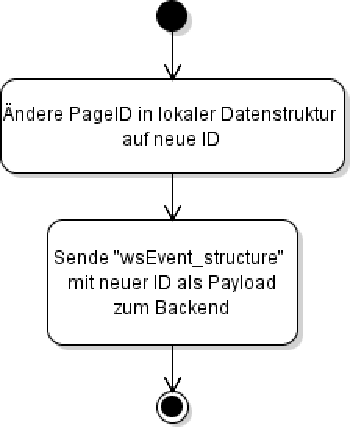
\includegraphics[width=\textwidth]{content/hauptteil/systemEntwurf/res/wsHandler/frontend/wsEvent_pageChange.pdf}
      \caption{WebsocketEvent:\\\emph{PageChange} empfangen}
      \label{fig:aDDF:wsEvent_pageChange}
  \end{subfigure}
  \hfill
  \begin{subfigure}[b]{0.38\textwidth}
      \centering
      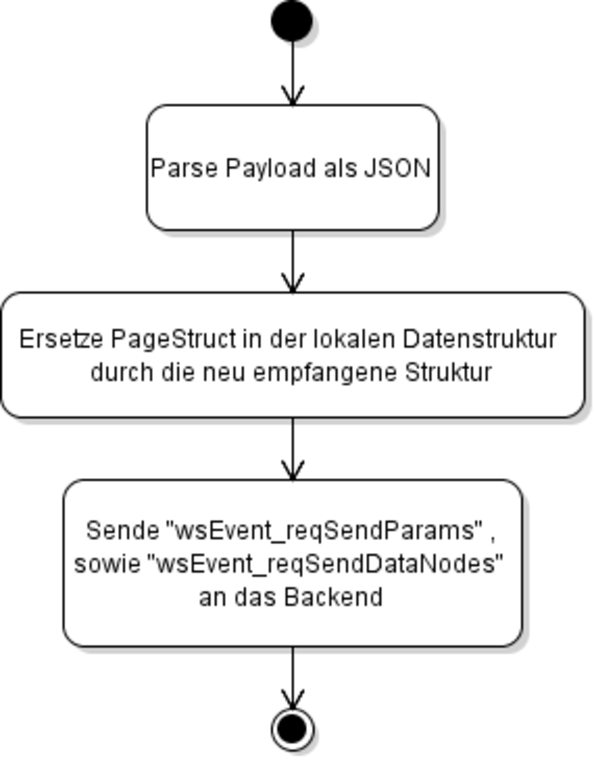
\includegraphics[width=\textwidth]{content/hauptteil/systemEntwurf/res/wsHandler/frontend/wsEvent_structure.pdf}
      \caption{WebsocketEvent:\\\emph{Structure} empfangen}
      \label{fig:aDDF:wsEvent_structure}
  \end{subfigure}
  \hfill
  \begin{subfigure}[b]{0.30\textwidth}
      \centering
      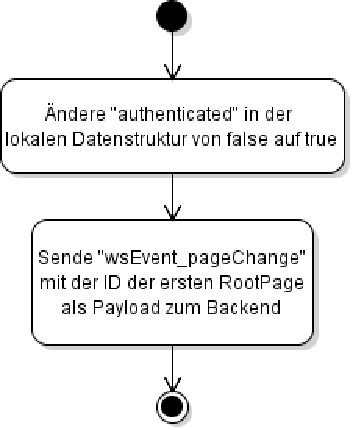
\includegraphics[width=\textwidth]{content/hauptteil/systemEntwurf/res/wsHandler/frontend/wsEvent_authentification.pdf}
      \caption{WebsocketEvent:\\\emph{Authentification} empfangen}
      \label{fig:aDDF:wsEvent_authentification}
  \end{subfigure}
     \caption[Aktivitätsdiagramme Dispatcher Frontend]{Aktivitätsdiagramme des Dispatchers im Frontend}
     \label{fig:activityDiagramDispatcherFrontend}
\end{figure}



\begin{figure}
  \centering
  \begin{subfigure}[b]{0.55\textwidth}
    \centering
    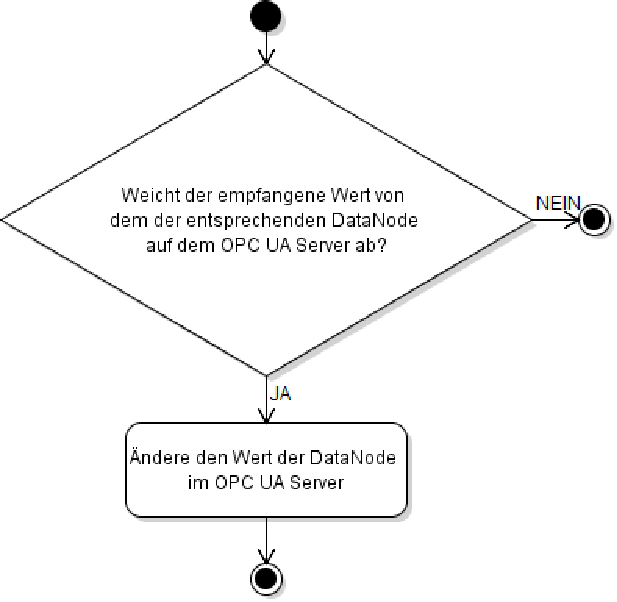
\includegraphics[width=\textwidth]{content/hauptteil/systemEntwurf/res/wsHandler/backend/wsEvent_dataNodeChange.pdf}
    \caption{WebsocketEvent:\\\emph{DataNodeChange} empfangen}
    \label{fig:aDDB:wsEvent_dataNodeChange}
  \end{subfigure}
  \hfill
  \begin{subfigure}[b]{0.49\textwidth}
      \centering
      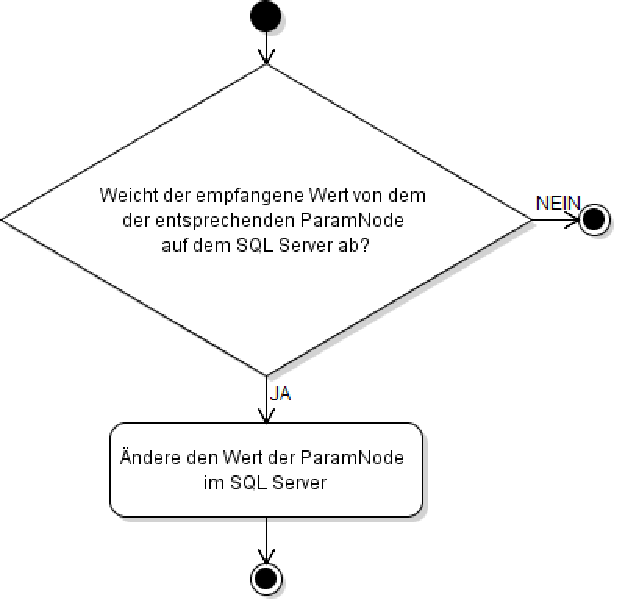
\includegraphics[width=\textwidth]{content/hauptteil/systemEntwurf/res/wsHandler/backend/wsEvent_paramNodeChange.pdf}
      \caption{WebsocketEvent:\\\emph{ParamNodeChange} empfangen}
      \label{fig:aDDB:wsEvent_paramNodeChange}
  \end{subfigure}
  \caption[Aktivitätsdiagramme Dispatcher Backend I]{Aktivitätsdiagramme des Dispatchers im Backend}
  \label{fig:activityDiagramDispatcherBackend}
\end{figure}

  
\begin{figure}
  \centering
  \begin{subfigure}[b]{0.48\textwidth}
    \centering
    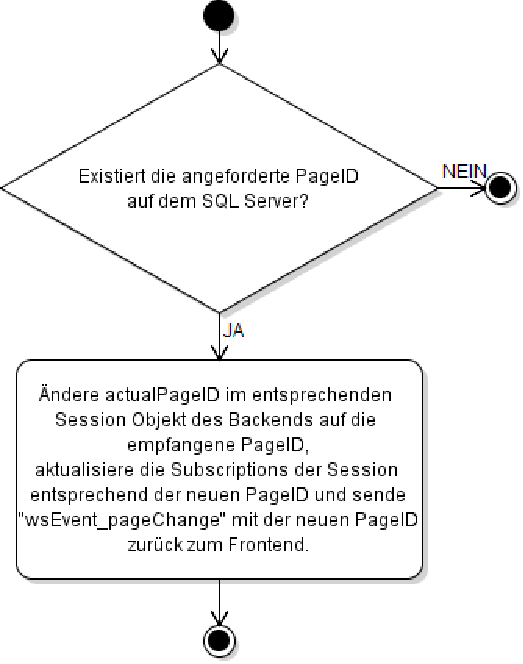
\includegraphics[width=\textwidth]{content/hauptteil/systemEntwurf/res/wsHandler/backend/wsEvent_pageChange.pdf}
    \caption{WebsocketEvent:\\\emph{PageChange} empfangen}
    \label{fig:aDDB:wsEvent_pageChange}
  \end{subfigure}
  \hfill
  \begin{subfigure}[b]{0.48\textwidth}
    \centering
    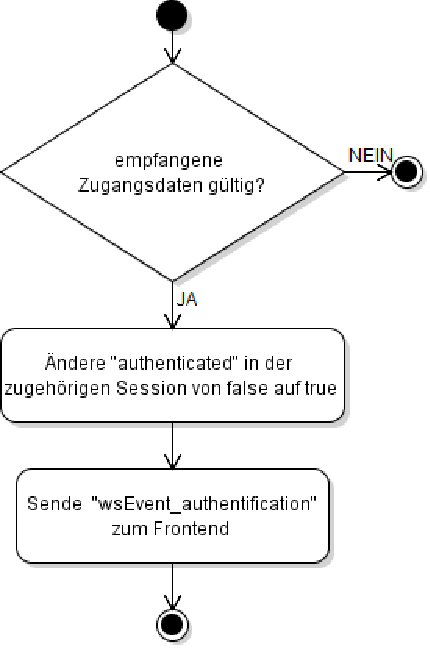
\includegraphics[width=\textwidth]{content/hauptteil/systemEntwurf/res/wsHandler/backend/wsEvent_authentification.pdf}
    \caption{WebsocketEvent:\\\emph{Authentification} empfangen}
    \label{fig:aDDB:wsEvent_authentification}
  \end{subfigure}
  \hfill
  \begin{subfigure}[b]{0.38\textwidth}
    \centering
    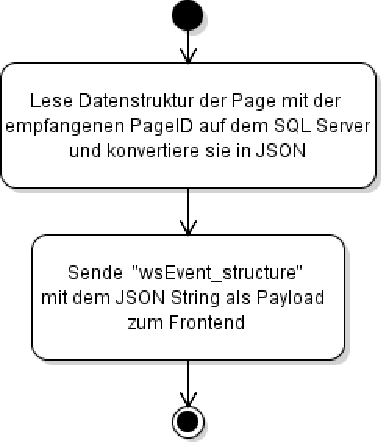
\includegraphics[width=\textwidth]{content/hauptteil/systemEntwurf/res/wsHandler/backend/wsEvent_structure.pdf}
    \caption{WebsocketEvent:\\\emph{Structure} empfangen}
    \label{fig:aDDB:wsEvent_structure}
  \end{subfigure}
  \caption[Aktivitätsdiagramm Dispatcher Backend]{Aktivitätsdiagramme des Dispatchers im Backend}
  \label{fig:activityDiagramDispatcherBackend}
\end{figure}